\documentclass[a4paper]{book}
%\pagestyle{page}
\usepackage{graphicx}
\usepackage{html}
\usepackage{ifpdf}
\usepackage{fancyhdr}
\usepackage[utf8]{inputenc}
\newcommand{\mbf}[1]{\mbox{\boldmath$#1$}}
\font\mbff=cmbsy10\def\mbfx#1{\hbox{\mbff#1}}%\let\mbf\Mbff
\newcommand{\del}[2]{\mbox{$\displaystyle\frac{#1}{#2}$}}
\newcommand{\pard}[2]{\del{\partial \,{#1}}{\partial \,{#2}}}
\newcommand{\ppd}[2]{\del{\partial \,{#1}}{\partial \,{#2}}}
\newcommand{\dpd}[2]{\del{\partial ^{2}\,{#1}}{\partial \,{#2}^{2}}}
\newcommand{\tpd}[2]{\del{\partial ^{3}\,{#1}}{\partial \,{#2}^{3}}}
\newcommand{\cpd}[2]{\del{\partial ^{4}\,{#1}}{\partial \,{#2}^{4}}}
%\newcommand{\spd}[1]{\del{\partial ^{3}\,{#1}}{\partial \,x\,\partial \,t^{2}}}
%\newcommand{\scpd}[1]{\del{\partial ^{4}\,{#1}}{\partial \,x^{2}\,\partial
%\,t^{2}}}
\newcommand{\der}[2]{\del{d \,{#1}}{d \,{#2}}}
\newcommand{\dd}[2]{\del{d ^2\,{#1}}{d \,{#2}^2}}
\newcommand{\td}[2]{\del{d ^3\,{#1}}{d \,{#2}^3}}
\newcommand{\cd}[2]{\del{d ^4\,{#1}}{d \,{#2}^4}}
\newcommand{\MKP}{{MKP$\;\;$}}
\newcommand{\inl}[2]{\mbox{$\displaystyle\int_{#1}^{#2}$}}
\newcommand{\sul}[2]{\mbox{$\displaystyle\sum_{#1}^{#2}\,$}}
\newcommand{\limit}[1]{\mbox{$\displaystyle\lim_{#1}$}}
\newcommand{\vp}{\varphi}
\newcommand{\e}{\mbf{\varepsilon}}
\newcommand{\ep}[0]{\mbf{\varepsilon}^p}
\newcommand{\epd}[0]{\dot{\mbf{\varepsilon}}^p}
\newcommand{\sig}{\mbf{\sigma}}
\newcommand{\sigs}{\sigma}%scalar
\newcommand{\kap}{\mbf{\kappa}}

\newcommand{\vsigrate}{\dot {\mbf{\sigma}}}
\newcommand{\sigrate}{\dot {\sigma}}
\newcommand{\taurate}{\dot {\tau}}
\newcommand{\erate}  {\dot {\mbf{e}}}

\newcommand{\rest}[1]{\Re\left( {#1} \right)}
\newcommand{\refeq}[1]{Eq.~(\ref{#1})}
\newcommand{\reffig}[1]{Fig.~(\ref{#1})}
\newcommand{\refeqs}[2]{Eqs.~(\ref{#1}), (\ref{#2})}
\newcommand{\refeqsr}[2]{\mbox{Eqs.~(\ref{#1})-(\ref{#2})}}

\newcommand{\C}{$^{\circ}\mathrm{C}$}
\newcommand{\ymu}{y_{\mu}}
\newcommand{\y}[1]{y_{#1}}
\newcommand{\ymui}[1]{y_{\mu_{#1}}}
\newcommand{\tdymu}{{\dot y}_{\mu}}
\newcommand{\ttdymu}{{\ddot y}_{\mu}}
\newcommand{\timeder}[1]{\dot {#1}} 
\newcommand{\dprime}{\prime\prime}

\newcommand{\beq}{\begin{equation}}
\newcommand{\eeq}{\end{equation}}
\newcommand{\bea}{\begin{eqnarray}}
\newcommand{\eea}{\end{eqnarray}}
\newcommand{\vsi}{\mbf{\sigma}}
\newcommand{\vep}{\mbf{\varepsilon}}
\newcommand{\eps}{\varepsilon}
\newcommand{\mD}{\mbf{D}}
\newcommand{\vxi}{\mbf{\xi}}
\newcommand{\vx}{\mbf{x}}
\newcommand{\dxi}{\;\mbox{d}\mbf{\xi}}
\newcommand{\vf}{\mbf{f}}
\newcommand{\vg}{\mbf{g}}
\newcommand{\veps}{\mbf{\varepsilon}}
\newcommand{\mB}{\mbf{B}}
\newcommand{\vsig}{\mbf{\sigma}}
\newcommand{\vd}{\mbf{d}}
\newcommand{\mK}{\mbf{K}}
\newcommand{\macbra}[1]{\langle{#1}\rangle}
\newcommand{\vbs}{\mbf{b}^{\sigma}}
\newcommand{\vbe}{\mbf{b}^{\eta}}
\newcommand{\vbeT}{\mbf{b}^{\eta T}}

\newcommand{\ud}{\mathrm{d}}
\newcommand{\grad}{\nabla}
%position vectors
\newcommand{\x}{\mbf{x}}
\newcommand{\xd}{\mbf{x}^\varphi}
%displacement
\newcommand{\du}{\mbf{u}} 
\newcommand{\bestresultcolor}{blue}
\newcommand{\bestresult}[1]{\textcolor{\bestresultcolor}{\bf{#1}}}
\newcommand{\ignore}[1]{}





\newcommand{\oofem}{\htmladdnormallink{OOFEM}{http://www.oofem.org}\ }
\newcommand{\oofemlnk}[1]{\htmladdnormallink{#1}{http://www.oofem.org}\ }
\newcommand{\bp}{\htmladdnormallink{Bo\v{r}ek Patz\'{a}k}{http://mech.fsv.cvut.cz/~bp/bp.html}}



\oddsidemargin -10mm
\evensidemargin -10mm
\textwidth 180mm
\parindent 0mm

\begin{document}
%begin{latexonly}
\title{
\ifpdf
\oofemlnk{\centerline{
\includegraphics[width=0.7\textwidth]{figs/oofem-logo-contour.pdf}}}
\else
\oofemlnk{\centerline{
\includegraphics[width=0.7\textwidth]{figs/oofem-logo-contour.eps}}}
\fi
Theory manual}
\author{Bořek Patzák, Martin Horák, Filip Kolařík\\ \\
Czech Technical University\\
Faculty of Civil Engineering\\
Department of Structural Mechanics\\
Th\'akurova 7, 166 29 Prague, Czech Republic
}
\maketitle
%end{latexonly}
\begin{htmlonly}
\begin{center}
\oofemlnk{\centerline{
\includegraphics[width=0.7\textwidth]{figs/oofem-logo-contour.eps}}}
{\Large Theorz manual}\\ \\
{Bořek Patzák, Martin Horák, Filip Kolařík\\ 
Czech Technical University\\
Faculty of Civil Engineering\\
Department of Structural Mechanics\\
Th\'akurova 7, 166 29 Prague, Czech Republic
}
\end{htmlonly}

\section*{Acknowledgments}
This work was supported by the Grant Agency of the Czech Republic -
Project No.: 103/97/P106.

\clearpage
\setcounter{page}{1}
\pagestyle{headings}

\tableofcontents
\chapter{Introduction and basic equations}
\section{Introduction}
% Section: Introduction
The aim of this document is to ducument the theoretical bacground of available solvers, elements, and models in oofem. At present, this manual is a working document, covering only small portion of its capabilities.  

\section{Notation}
\section{Basic equations}
% Basic equations
\section{Linear elasticity}
\subsection{Linear kinematics}
Let us consider a deformable body as a collection of points, where position of each point is denoted as $\x\in\Omega$. In a deformed configuration the position of each point is identified by its position vector $\xd(x) = \mbf{\phi}(\x)$. The displacement vector is then defined as:
\begin{equation}
  \label{eq:displacementvector}
  \xd(\x) = \x + \du(\x)  
\end{equation}

Let us now examine the position in a local neighborhood of a point. The deformed position of such neighbor point with coordinates $\x+d\x$ (where d\x is infinitisemally small vector) is
$$\xd(\x+d\x) = \x+d\x+\du(\x+d\x) = \xd + d\xd$$,
where $d\xd$ is the mapping of vector $d\x$ onto deformed configuration, see Fig.~\ref{fig:deformedconfiguration}.
\begin{figure}
  \begin{center}
    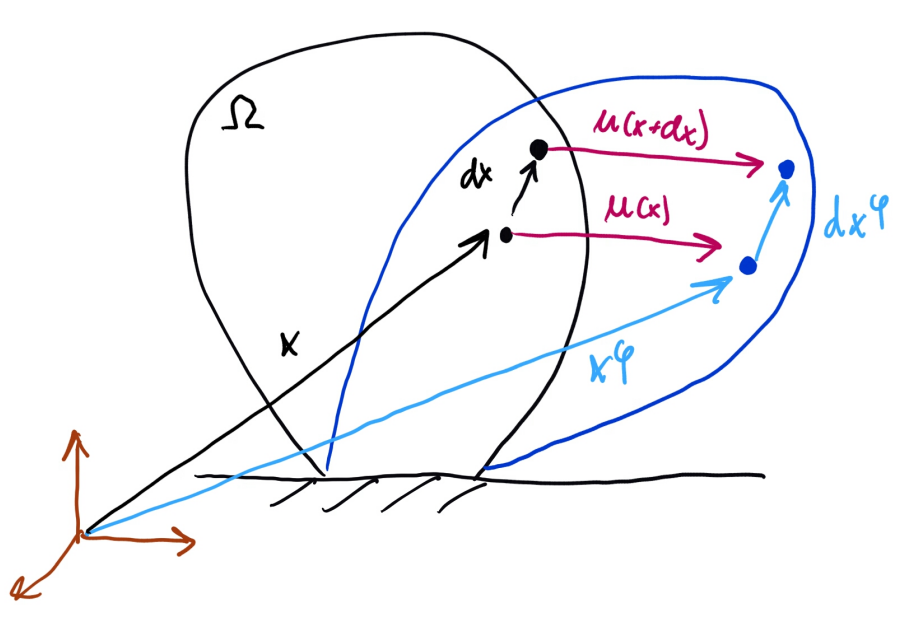
\includegraphics[width=0.5\textwidth]{figs/deformedconfiguration.png}
  \end{center}
  \label{fig:deformedconfiguration}
  \caption{Deformed configuration}
\end{figure}
Taking into account the definition of displacement vector ~\ref{eq:displacementvector} and using Taylor formula we get
\begin{equation}
  d\xd = \x+d\x+\du(\x+d\x)-\xd = d\x-\du(\x)+\du(\x+d\x) \approx [\mbf{I}+\grad\du(\x)]d\x
\end{equation}
where $\grad\du(\x)$ is the displacement gradient tensor (in small strain theory we assume $\vert\vert\grad\du(\x)\vert\vert \ll 1$).
The displacement gradient tensor can be decomposed into symetric and antisymmetric parts
$$
\grad\du = \mbf{\eps}+\mbf{\omega}={1\over 2}(\grad\du+\grad\du^T)+{1\over 2}(\grad\du-\grad\du^T) = \grad^s\mbf{u}+\grad^a\mbf{u}
$$

The antisymmetric part corresponds to infinitesimal rotation. The symmeric part of displacement gradient tensor is therefore the measure of infinitesimal deformation
$$
d\xd = \mbf{\eps} d\x
$$
\subsection{Equlibrium equations}
Stress is defined as the force across a "small" boundary per unit area of that boundary, for all orientations of the boundary. In the most general case, called triaxial stress, the stress is nonzero across every surface element. Cauchy observed that the stress vector $\mbf{t}$ across a surface is a linear function of the surface's normal vector $\mbf{n}$:
$$
\mbf{t}(x)=\mbf{\sigma}(x)\mbf{n}(x)
$$
where $\mbf{\sigma}(x)$ is called the (Cauchy) stress tensor, completely describing the stress state at any point.
\begin{figure}
  \begin{center}
    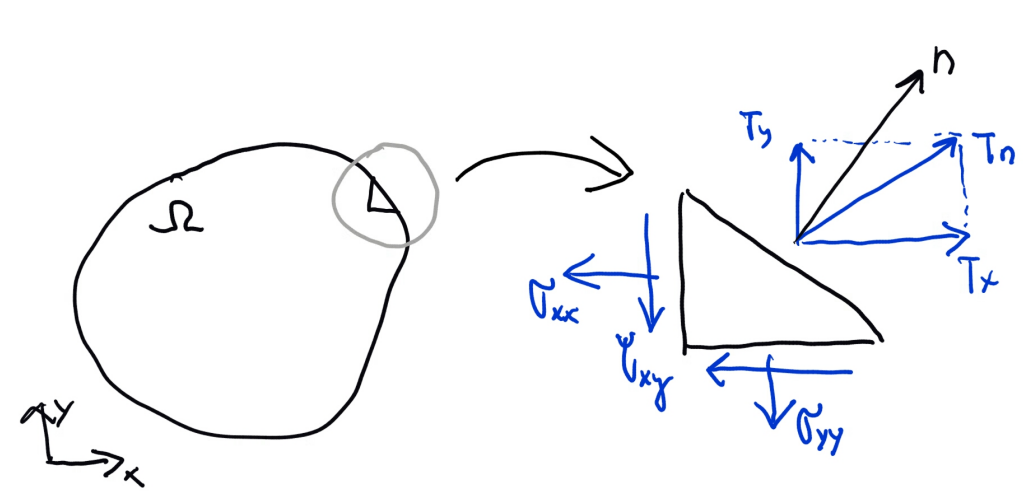
\includegraphics[width=0.5\textwidth]{figs/tractionstressrelation.png}
  \end{center}
  \label{fig:tractionstressrelation}
  \caption{Balance between tractions and stresses in 2D}
\end{figure}

The components of the Cauchy stress tensor at every point in a material satisfy the equilibrium equations (Cauchy’s equlibrium equations). From the conservation of angular momentum follows the symmetry of the stress tensor. Therefore, the stress state of the medium at any point and instant can be specified by only six independent parameters, rather than nine. These may be written
$$
\left[
  \begin{array}{ccc}
    \sigma_{xx} & \tau_{xy} & \tau_{xz}\\
    \tau_{xy} & \sigma_{yy} & \tau_{yz}\\
    \tau_{zx} & \tau_{zy} & \sigma_{zz}
  \end{array}
\right] 
$$
where the elements $\sigma_{xx}, \sigma_{yy}, \sigma_{zz}$ are called the normal stresses (relative to the chosen coordinate system), and $\tau_{yz}, \tau_{xz}, \tau_{xy}$ the shear stresses.

In a static equlibrium, the Cauchy stress components in every material point satisfy the equilibrium equations, see~ref{fig:stressbalance}
\begin{equation}
  \sigma_{ji, j} + F_i = 0
\end{equation}
where we use summation convention over repated indices and $F_i$ are the components of the body force. In a compact tensorial notation we can write the above equation as
\begin{equation}
  \grad\cdot\sigma + F_i = 0
  \label{eq:staticequlibruim3d}
\end{equation}

\begin{figure}
  \begin{center}
    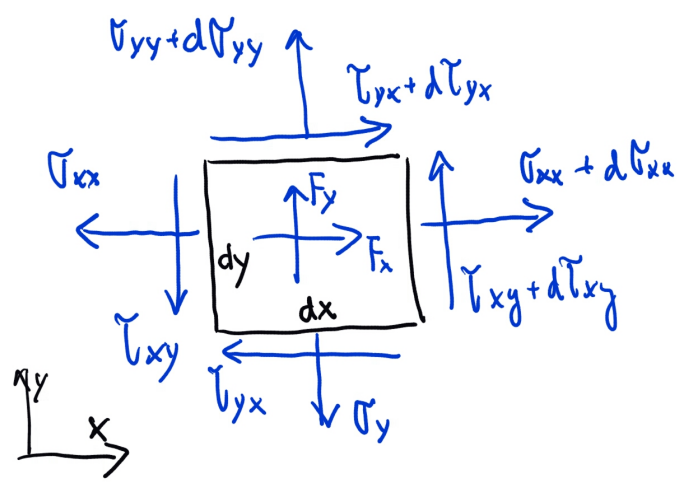
\includegraphics[width=0.5\textwidth]{figs/stressbalance2d.png}
  \end{center}
  \label{fig:stressbalance}
  \caption{Stress balance in 2D}
\end{figure}

\subsection{Constitutive equations}
In this section we present the constituve relations (i.e. relations between stress and strain tensors) for the case of hyperelasticity, which could be defined in terms of strain energy density $W(\mbf{\eps})$, which allows to evaluate stress components as partial derivatives:
$$
\sigma_{ij}=\pard{W}{\eps_{ij}}
$$
For example, the Hooke's law  is defined using following strain energy potential
$$
W(\eps) = \del{1}{2}\eps_{ij}\mbf{C}_{ijkl}\eps_{kl}
$$
where $\mbf{C}$ is forth order elasticity tensor. The equality of mixed derivatives $(\dpd{W}{\eps_{ij}\eps_{kl}} = \dpd{W}{\eps{kl}\eps{ij}})$ and symmetry of stress and strain tensors $\pard{\sigma{ij}}{\eps_{kl}} = C_{ijkl}=C_{jikl}=C_{ijlk}$ imply that there is in general maximum 21 independ components of the elasticity tensor.
In the simplest case, the elasticity tensor for isotropic linear elastic material  can be described by only two parameters: either Lame\'s parameters ($\lambda, \mu$) or more usual parametrs being Young's modulus $E$ and Poisson's ratio $\nu$:
$$
C_{ijkl}=\lambda\delta_{ij}\delta_{kl}+2\mu {1\over 2}[\delta_{ik}\delta_{jl}+
 \delta_{il}\delta_{jk}] \equiv \mbf{C}=\lambda\mbf{1}\otimes\mbf{I}+2\mu\mbf{I}
$$

\subsection{Voight notation}

The Voigt notation is hrequantly used to take advantage of the symmetry of the stress tensor to express the stress tensor as a six-dimensional vector of the following form:
$$
\tilde{\mbf{\sigma}}=
\left[
  \sigma_{x}, \sigma_y, \sigma_z, \tau_{yz}, \tau_{xz}, \tau_{xy}
  \right]^T \equiv
\left[
  \sigma_{xx}, \sigma_{yy}, \sigma_{zz}, \tau_{yz}, \tau_{xz}, \tau_{xy}
  \right]^T
$$

The strain tensor, similar in nature to the stress tensor (both symmetric second-order tensors) can be written in Voight notation as
$$
\tilde{\mbf{\eps }}=
\left[
  \eps_{x}, \eps_y, \eps_z, \gamma_{yz}, \gamma_{xz}, \gamma_{xy}
  \right]^T \equiv
\left[
  \eps_{xx}, \eps_{yy}, \eps_{zz}, 2\eps_{yz}, 2\eps_{xz}, 2\eps_{xy}
  \right]^T
$$

The benefit of using different representations for stress and strain is the scalar invariance
$$
\mbf{\sigma}\cdot\mbf{\eps}=\sigma_{ij}\eps_{ij}=\tilde{\sigma} \tilde{\eps}
$$
Similarly, a three-dimensional symmetric fourth-order tensor can be reduced to a [6,6] matrix.


\subsection {Boundary value problem in small strain elasticity}
\subsubsection{Strong form}

Starting from the equilibrium equations~ref{eq:staticequlibrium3d}, into which we can substitute the constituve equations and strain-displacement relation we obtain the equlibrium equation expressed in terms of displacements:
$$
\pard{}{x_j}\left({C_{ijkl} {1\over 2}(\pard{u_k}{x_l}+\pard{u_l}{x_k})}\right) + F_i = 0
$$
This system of three partial differnetial equations can be solved, provided that appropriate boundary conditions are given. In summary, the strong form is the following:\\
\begin{center}
\fbox{
  \begin{minipage}{8cm}
    Find $\mbf{u}\in R^n$, such that\\[4mm]
    $\pard{}{x_j}\left({C_{ijkl} {1\over 2}(\pard{u_k}{x_l}+\pard{u_l}{x_k})}\right) + F_i = 0 \in \Omega\,$\\[2mm]
    $\mbf{u}=\mbf{\bar{u}} \in \Gamma_u$\\[2mm]
    $\mbf{t}^n_i = C_{ijkl}{1\over 2}(\pard{u_k}{x_l}+\pard{u_l}{x_k})\,n_j = \bar t_i \,\in \Gamma_t$
  \end{minipage}
}
\end{center}

\subsubsection{Weak form}

  By following the method of weighted residuals, we multiply the governing differential equations~\ref{eq:equlibriumequations3d} in residual form by a sutable test functions $\delta\mbf{u}$, satisfying the homogeneous boundary conditions on $\Gamma_u$
  $$
  \int_\Omega \delta\mbf{u} \cdot \left(
  \grad\cdot\mbf{\sigma} + F \right)\ d\Omega = \mbf{0}
  $$
  By applying the Green's formula, we arrive at
  $$
  \int_\Omega\grad\delta\mbf{u}\cdot\mbf{\sigma}\ d\Omega =
  \int_\Omega\delta\mbf{u}\cdot\mbf{F}\ d\Omega + \int_\Gamma\delta\mbf{u}\cdot\mbf{\sigma}\mbf{n}\ d\Gamma
  $$
  Then we can substitute for the stresses and tractions and taking into account the symmetry of stress tensor ($\sigma=C\mbf{\eps})$
  \begin{equation}
  \int_\Omega\grad^s\delta\mbf{u}\cdot\mbf{C}\mbf{\eps}\ d\Omega =
  \int_\Omega\delta\mbf{u}\cdot\mbf{F}\ d\Omega + \int_\Gamma\delta\mbf{u}\cdot\mbf{t}\ d\Gamma
  \label{weakform3d}
  \end{equation}
  Or, equaivalently using Voight's notation
  \begin{equation}
  \int_\Omega\delta\tilde{\eps}^T\tilde{\mbf{D}}\tilde{\mbf{\eps}}\ d\Omega =
  \int_\Omega\delta\mbf{u}^T\mbf{F}\ d\Omega + \int_\Gamma\delta\mbf{u}^T\mbf{t}\ d\Gamma
  \label{eq:weakformvoight}
  \end{equation}
  
  Note: this is equaivalent to the principle of virtual displacements. For hyperelastic material, the weak form is identical to the principle of minimum potential energy.

  
\subsection{Finite element discretization}
Let us consider discretization of the problem domain $\Omega$ into set of nonoverlapping subdomains $\Omega_e$, called elements.
Next we will consider the approximation of the unknown displacement field, defined on individual subdomains. Note that the approximation is not arbitrary:
\begin{itemize}
  \item The weak form kontains only first derivatives of the unknown and test functions, thus only $C^0$ continuity is required.
\end{itemize}
The element approxiamtion of the arbitrary function $f$ has the form
$$
f = \sum N_j(\mbf{x})r_j  = \mbf{N}\mbf{r}
$$
where $N_j$ are so called shape or approximation functions and $r_j$ are nodal values.
Note that for the approximation functions to be interpolatory, the shape functions have to satisfy Kronecker-delta property, i.e., $N_j(\mbf{x}_i)=\delta_{ij}$, where $\mbf{x}_i$ is the position vector of the i-th node. Also, the shape functions have to satisfy the condition $\sum N_i=1$, which follows from the requirement to approximate the constant function.
The required continuity of element approximations have to be satisfied. This is typically achieved by enforcing the continuity at the nodal points.
In our case, the approximation of displacements and test functions is
\begin{eqnarray}
  \mbf{u}^e&=&\mbf{N}^e(\mbf{x})\mbf{r}^e\\
  \delta\mbf{u}^t&=&\mbf{N}^e(\mbf{x})\delta\mbf{r}^e
\end{eqnarray}

We will use the weak form~\ref{weakform3d}, which using Voight's notation has the form
$$
  \int_\Omega\grad^s\delta\mbf{u}\cdot\mbf{C}\mbf{\eps}\ d\Omega =
  \int_\Omega\delta\mbf{u}\cdot\mbf{F}\ d\Omega + \int_\Gamma\delta\mbf{u}\cdot\mbf{t}\ d\Gamma
$$

  We will need also the derivatives of the displacement and test functions
  \begin{eqnarray}
  \tilde{\eps}^e = = \mbf{B}^e(\mbf{x})\mbf{r}^e\\
  \delta\tilde{\eps}^e&=&\mbf{B}^e(\mbf{x})\delta\mbf{r}^e
\end{eqnarray}
where $B^e$ matrix contains the first partial derivatives of the shape functions. 
By substiituting into the weak form~\ref{eq:weakformvoight} we obtain
\begin{equation}
  \sum_e \delta\mbf{r}^{e,T}
  \left[
    \underbrace{\int_{\Omega^e} \mbf{B}^{e,T}\tilde{\mbf{D}}^e\mbf{B}^e\mbf{r}^e\ d\Omega}_{\mbf{K}^e}\mbf{r}^e-\underbrace{\int_{\Omega}\mbf{N}^{e,T}\mbf{F}\ d\Omega}_{\mbf{f}^e_\Omega} - \underbrace{\int_{\Gamma_t}\mbf{N}^{e,T}\bar{\mbf{t}}\ d\Gamma}_{\mbf{f}^e_\Gamma}
    \right] = \mbf{0}
\end{equation}

After introducing a mappig between element displacement vectors $\mbf{r}^e$, nodal vectors of test function values $\delta\mbf{r}$ and their global counterparts $\hat{\mbf{r}}, \delta\hat{\mbf{r}}$ one can obtain
\begin{equation}
  \delta\hat{\mbf{r}}^{T}
  \left[
    \hat{\mbf{K}}\hat{\mbf{r}}-\hat{\mbf{f}}_\Omega - \hat{\mbf{f}}_{\Gamma}
    \right] = \mbf{0}
\end{equation}
By taking into account that the test fuctions are arbitrary (i.e. $\delta\hat{\mbf{r}}\ne\mbf{0}$), one finnaly obtains the following set of linear algebraic equations for unknonwn nodal displacements $\hat{\mbf{r}}$:
\begin{equation}
    \hat{\mbf{K}}\hat{\mbf{r}}=\hat{\mbf{f}}_\Omega + \hat{\mbf{f}}_{\Gamma}
\end{equation}



\chapter{Solution procedures}
\section{Transient incompressible flow\\PFEM Algorithm}
\subsection{Lagrangian governing equations of incompressible fluid}
The Particle finite element method (PFEM) is based on the Lagrangian form of the Navier-Stokes equation for incompressible Newtonian fluids. Assuming the density does not change in time for an incompressible fluid, the continuity equation reduces to zero requirements for the divergence of the velocity. The Navier-Stokes equations take the form
\begin{eqnarray}
\rho\pard{\mbf{u}}{t} &=& \rho\mbf{b} + \nabla\cdot\mbf{\sigma} \label{eq:navier-stokes2}\;,\\
\nabla\cdot\mbf{u} &=& 0\;. \label{eq:navier-stokes2b}
\end{eqnarray}
For the deviatoric stress in Newtonian fluids a linear dependency of stress tensor and strain rate tensor is adopted and for the Newtonian fluids. Considering the incompressibility of the fluid, the Cauchy stress reads
\begin{equation}\label{eq:stokes}
\mbf{\sigma}=-p\mbf{I} + 2\mu \nabla^s\mbf{u}\;.
\end{equation}
This equation is known as \emph{Stokes' law} and its Cartesian form writes
\begin{equation}
\sigma_{ij}=-p\delta_{ij}+\mu\left(\pard{u_i}{x_j}+\pard{u_j}{x_i}\right)\;.
\end{equation}
\par
Substituting the expression of Cauchy stress from Stokes' law~(\ref{eq:stokes}) into the momentum equation~(\ref{eq:navier-stokes2}) and rewriting gives
\begin{equation}
\rho\pard{\mbf{u}}{t} = \rho\mbf{b} + \mu\nabla^2\mbf{u} - \nabla p\;.\label{eq:momentum}
\end{equation}
\par
The governing equations of the mass~(\ref{eq:navier-stokes2b}) and momentum conservation~(\ref{eq:momentum}) form can be written in the Cartesian form for the individual component $i$ using Einstein summation convention
\begin{eqnarray}
\rho \pard{u_i}{t} &=& - \frac{\partial}{\partial x_i}p+\mu\frac{\partial}{\partial x_j}\left(\frac{\partial u_i}{\partial x_j}\right)+\rho b_i \;, \label{eq:mb}\\
\pard{u_i}{x_i} &=& 0\;.
\end{eqnarray}
The equations are accompanied by a set of standard boundary conditions imposed on the complementary parts of the domain boundary
\begin{eqnarray}
  \tau_{ij}\nu_j - p\nu_i &=& \bar \sigma_{ni} \qquad \mbox{on } \Gamma_{\sigma}\;, \\
  u_i\nu_i &=& \bar u_n \qquad\; \mbox{on } \Gamma_n\;, \\
  u_i\zeta_i &=& \bar u_t \qquad\;\, \mbox{on } \Gamma_t\;,
\end{eqnarray}
where $\nu$ or $n$ denotes the normal direction to the boundary and $\zeta$ or $t$ the tangential one. The bar sign over a quantity $\bar x$ stands for its prescribed value.

\subsection{Time discretization}
For the time discretization of the momentum equation, a general trapezoid rule can be adopted. Using this rule, the time derivative of a generic function $\phi$ can be approximated by following equation
\begin{equation}
[\phi(x,t)]^{n+\theta} = \theta\phi(x,t^{n+1})+(1-\theta)\phi(x,t^n)=\theta\phi^{n+1}+(1-\theta)\phi^n\;.
\end{equation}
Rewriting the time derivative on the left hand side of the momentum balance~(\ref{eq:mb}) as a finite difference in time and applying the trapezoidal rule on the right hand side, we obtain
\begin{equation}\label{eq:momentum-general}
  \rho\pard{u_i}{t} \approx \rho\frac{u^{n+1}_i-u^n_i}{\Delta t}= \left[ - \frac{\partial}{\partial x_i}p+\mu\frac{\partial}{\partial x_j}\left(\frac{\partial u_i}{\partial x_j}\right)+\rho b_i\right]^{n+\theta}\;.
\end{equation}
The parameter $\theta$ can take values from the interval $[0,1]$.  The approximation is considered as a weighted average of the derivative values in the time step $n$ and $n+1$. Using a specific value of the $\theta$ parameter, well-known methods can be recovered: The explicit Euler method $\theta=0$, the backward Euler for $\theta=1$ or the Crank-Nicolson method $\theta=1/2$. The current implemantation of PFEM allows the use of explicit and backward (implicit) method.

\subsection{Fractional step scheme}
Beside the three velocity components, the discretized momentum balance equations~(\ref{eq:momentum-general}) for a three dimensional case includes pressure as a coupling variable. A possible approach to decouple them is the application of so-called \emph{fractional step method}. The main idea of this method consists in introducing an intermediate velocity as supplementary variable and splitting the momentum equation. The modification introduced by R.Codina~\cite{Codina01} splits the the discretized time step is split into two sub-steps. The implicit part of the pressure is avoided and assigned to the second step.
\begin{equation}
  \pard{u_i}{t} \approx \frac{u^{n+1}_i-u^n_i}{\Delta t}=\frac{u^{n+1}_i-u^*_i+u^*_i-u^n_i}{\Delta t}= \left[ - \frac{1}{\rho}\frac{\partial}{\partial x_i}p+\frac{\mu}{\rho}\frac{\partial}{\partial x_j}\left(\frac{\partial u_i}{\partial x_j}\right)+b_i\right]^{n+\theta}\;.
\end{equation}
where the intermediate velocity $u^*_i$ is introduced. Splitting the equation in the following manner gives the expression for the unknown velocities
\begin{eqnarray}\label{rce:uistar}
    u^*_i &=& u^n_i+b_i\Delta t - \frac{\Delta t}{\rho}\pard{}{x_i}\gamma p^n+\frac{\Delta t\mu}{\rho}\pard{}{x_j}\left(\pard{u^{n+\theta}_i}{x_j}\right)\;,\\
    u^{n+1}_i &=& u^*_i- \frac{\Delta t}{\rho}\pard{}{x_i}(p^{n+1}-\gamma p^n)\;. \label{eq:uin1}
\end{eqnarray}

The pressure split is here introduced by the new parameter $\gamma$ defining the amount of splitting and can take values from 0 to 1. The body loads are considered to be constant over time step.
\par
In a similar way, the fractional step method is applied on the mass conservation equation. Here, the time derivative of density would be approximated. As we examine an incompressible flow, whose density does not change in time, merely the intermediate velocity term is incorporated in the divergence of the velocity.
\begin{equation}
  \pard{(u^{n+1}_i-u^*_i+u^*_i)}{x_i} = 0 \;,
\end{equation}
which can be decomposed into two sub-equations

\begin{eqnarray}\label{rce:mass}
	\pard{u^*_i}{x_i} &=& 0 \\
      \pard{(u^{n+1}_i-u^*_i)}{x_i} &=& 0\;.
\end{eqnarray}

By substituting for the velocity difference into the equation~(\ref{eq:uin1}) we obtain
\begin{equation}
\pard{}{x_i}(u^{n+1}_i - u^*_i) = \pard{}{x_i}\left(-\frac{\Delta t}{\rho}\pard{}{x_i}(p^{n+1}-\gamma p^n)\right)\;.
\end{equation}
Now we can sum the separated mass equations together. This operation gives the coupled mass-momentum equation
\begin{equation}
  \pard{u^*_i}{x_i} - \frac{\Delta t}{\rho}\frac{\partial^2}{\partial x^2_i}(p^{n+1}-\gamma p^n) = 0\;.
\end{equation}
The final set of equations reads
\begin{eqnarray}
u^*_i  &=& u^n_i+b_i\Delta t - \frac{\Delta t}{\rho}\pard{}{x_i}\gamma p^n+\frac{\Delta t\mu}{\rho}\pard{}{x_j}\left(\pard{u^{n+\theta}_i}{x_j}\right)\;,\\
\frac{\partial^2}{\partial x^2_i}(p^{n+1}) &=& \frac{\rho}{\Delta t}\pard{u^*_i}{x_i}+\frac{\partial^2}{\partial x^2_i}(\gamma p^n)\;, \\
u^{n+1}_i &=& u^*_i- \frac{\Delta t}{\rho}\pard{}{x_i}(p^{n+1}-\gamma p^n)\;.
\end{eqnarray}
\par
The above PFEM formulation is based on the paper by Idelsohn, O\~nate and Del Pin~\cite{Idelsohn04}. The authors described an approach using arbitrary time discretization scheme and pressure split factor. Their choice of implicit scheme $\theta = 1$ was motivated by better convergence properties, whereas the decision for $\gamma = 0$ leading to greater pressure split was driven by better pressure stabilization.
\subsection{Spatial discretization}
The unknown functions of velocity and pressure are approximated using equal order interpolation for all variables in the final configuration
\begin{eqnarray}
u_i&=&\mbf{N}^T(X,t)\mbf{U}_i\\
p&=&\mbf{N}^T(X,t)\mbf{P} \;.
\end{eqnarray}
By applying the Galerkin weighted residual method on the splitted governing equations, following system of linear algebraic equations is obtained 
\begin{eqnarray}
\mbf{M}\mbf{U}^* &=& \mbf{M}\mbf{U}^n + \Delta t\mbf{F} - \frac{\Delta t\mu}{\rho}\mbf{K}\mbf{U}^{n+\theta}\;,\label{eq:systemA} \\
\mbf{L}\mbf{P}^{n+1} &=&\frac{\rho}{\Delta t}\left(\mbf{G}^T\mbf{U}^*-\hat{\mbf{U}}\right) \;, \label{eq:systemB} \\
\mbf{M}\mbf{U}^{n+1} &=& \mbf{M}\mbf{U}^* - \frac{\rho}{\Delta t}\mbf{G}\mbf{P}^{n+1} \;.\label{eq:systemC}
\end{eqnarray}
\par
The matrix $\mbf{M}$ denotes the mass matrix in a lumped form, whereas the vector $\mbf{F}$ stands for the load vector. The matrix $\mbf{G}$ represents the gradient operator, which is the transposition of the divergence operator denoted simply as $\mbf{G}^T$. Matrices $\mbf{K}$ and $\mbf{L}$ are build in a similar way however noted differently. Both mean the Laplacian operator. Due to its common use in computational mechanics, the classical notation of the stiffness matrix $\mbf{K}$ is used. Prescribed velocity components are enclosed in vector $\hat{\mbf{U}}$.
\par
In each computational time step, an iteration is performed until the equilibrium is reached. Depending on the value of $\theta$ used, the equation system for the components of the auxiliary velocity $U^*_i$~(\ref{eq:systemA}) can be solved either explicitly $\theta = 0$ or implicitly $\theta \neq 0$. Then, the calculated values of the auxiliary velocity are used as input for the pressure computation~(\ref{eq:systemB}). The last system of equations~(\ref{eq:systemC}) determines the velocity values at the end of the time step, taking auxiliary velocities and pressure or pressure increments into account.
\par
Let us summarize the iterative step. The position of the particles at the end of the previous time step is known, as well as the the value of the velocity $u^n$ and pressure $p^n$. The set of governing equations is build up for the unknowns at the end of the solution step $\theta^{n+1}$, however based on the geometry of the previous step. The changes in the position are neglected. Once the convergence is reached, the final position is computed from the old one modified by the displacement due to obtained velocity. After that, solution can proceed to the next time step.

\chapter{Elements}
\chapter{Constitutive Equations}
\chapter{Boundary conditions}

\phantomsection
\addcontentsline{toc}{chapter}{Bibliography}

\bibliographystyle{plain}
\bibliography{references}

\end{document}


